\documentclass[a4paper,10pt]{article}
% Space around section titles
\usepackage{parskip}
% Required for specifying custom colors
\usepackage{xcolor}
% Used to customize the \section command
\usepackage{titlesec}
% Font
\usepackage{fontspec}
\setmainfont[Ligatures=TeX]{Roboto}
% Space around the page
\usepackage[left=1.9cm, right=1.9cm, top=1.1cm, bottom=1.0cm]{geometry}
% Custom links
\usepackage{hyperref}
% For right-aligned table column
\usepackage{array}
% For customizing itemize
\usepackage{enumitem}
% For including headshot picture
\usepackage{graphicx}
% For headshot picture positioning in table
\usepackage{multirow}
% For icons
\usepackage{fontawesome}

% Set link colors throughout the document
\hypersetup{colorlinks,
			breaklinks,
			urlcolor=linkcolour,
			linkcolor=linkcolour,
			pdfauthor={Babken Vardanyan},
			pdftitle={Babken Vardanyan's CV},
			pdfsubject={CV},
			pdfkeywords={Impressive, you can strip pdf metadata!}}
% Space length in tables
\setlength{\tabcolsep}{0.5em}
% Text formatting of sections
\titleformat{\section}{\Large\scshape\raggedright}{}{0em}{}[\titlerule]
% Spacing around sections
\titlespacing{\section}{0pt}{1.5pt}{1.5pt}
% Removes page numbering
\pagestyle{empty}
% Link color
\definecolor{linkcolour}{rgb}{0,0.2,0.6}
% Macro for URLs
\newcommand{\site}[2]{{\color{blue}{\texttt{\href{#1} {#2}}}}}


\begin{document}

\par{\centering{\Huge Babken Vardanyan}\bigskip\par}
\par{\centering{\Large Python Developer}\bigskip\par}

\begin{minipage}[t]{0.65\textwidth}
	\begin{tabular}{c l}
		\faMapMarker & Dro 16, Yerevan, Armenia \\
		\faEnvelope & \site{mailto:babkenvardanyan94@gmail.com}{babkenvardanyan94@gmail.com} \\
		\faPhone & \site{tel:+37498399434}{+374 98 399434} \\
		\faSkype & \site{skype:babkenvardanyan1}{babkenvardanyan1} \\
		\faLinkedin & \site{https://www.linkedin.com/in/babkenvardanyan}{linkedin.com/in/babkenvardanyan} \\
		\faGithub & \site{https://github.com/axper}{github.com/axper} \\
		\faStackOverflow & \site{https://stackoverflow.com/users/2529583/babken-vardanyan}{stackoverflow.com/users/2529583} \\
	\end{tabular}
\end{minipage}
\begin{minipage}[c]{0.35\textwidth}
	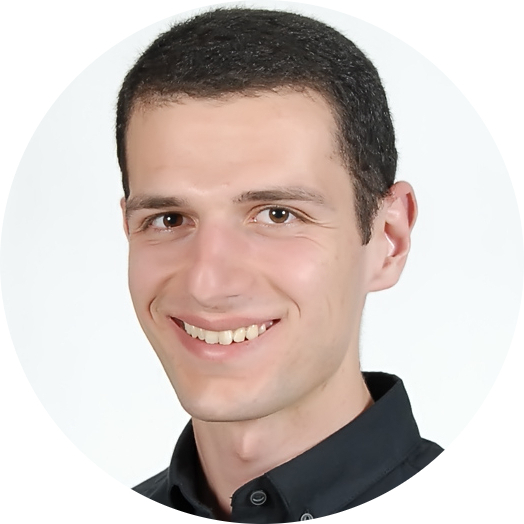
\includegraphics[height=75pt]{picture.jpg}
\end{minipage}


\section{Profile}

Python and Django developer with strong focus on delivery, stability and maintainability.
Proven track record of getting things done on time.
Effective and regular communication.
Knowledge of mulitple programming languages and frameworks.
Knowledge of server, database administration and information security.
I love to teach newcomers.
I adapt to new technologies quickly.
I love to tackle challenging technical problems.
I write docs and always test the code before pushing.


\section{Main Skills}

\begin{itemize}
\item \textsc{Python}: Django, REST Framework
\item \textsc{Java}: Android, Spring Framework, Hibernate, Junit, Mockito, Jersey
\item \textsc{Linux}: Bash, SystemD, Ansible, NginX, SSH, Docker, Kubernetes, VMWare
\item \textsc{Database}: SQL, Elasticsearch, MongoDB, SQLite
%\item \textsc{Editor}: Vim
\item \textsc{Other}: Selenium/Appium, iOS, Sonar, Nmap, Tcpdump, C, Powershell
\end{itemize}


\section{Work History}

\begin{itemize}
\item Overpass, \textbf{Lead Developer}, \site{https://app.getoverpass.com}{app.getoverpass.com} (Sep 2017 - Present)
\item Basic IT Center, \textbf{Programming Instructor}, \site{https://it-center.am}{it-center.am} (Sep 2017 - Present)
\item SFL LLC, \textbf{Java Developer}, \site{https://callmonkey.com}{callmonkey.com} (May 2015 - June 2017)
\item Unibank CJSC, \textbf{Security Administrator}, \site{http://unibank.am}{unibank.am} (May 2014 - May 2015)
\end{itemize}


\section{Professional Experience}

\begin{itemize}
\item Lead developer of Overpass, a lead capture app with Android, iOS, Django, Web codebases. Learned \mbox{Android} and iOS in just 1 week. Increased unit test coverage from 0 to 90\%:\\
	\site{https://app.getoverpass.com}{https://app.getoverpass.com}
\item Breaking down a monolith web app into microservices, complete rewrite from ground up with Java, Spring, MongoDB and Elasticsearch:\\
	\site{https://callmonkey.com}{https://callmonkey.com}
\item Development of distributed border security system for the Armenian Government:\\
	\site{https://sflpro.com/portfolio/2-5-million-border-checks-in-2015/}{https://sflpro.com/portfolio/2-5-million-border-checks-in-2015/}
\item Created a recipe sharing webside in under 48 hours during a hackathon:\\
	\site{https://hamegh.com}{https://hamegh.com}
\item Contributions to Open Source Documentation during spare time:\\
	\site{https://wiki.archlinux.org/index.php/Special:Contributions/Axper}{https://wiki.archlinux.org/index.php/Special:Contributions/Axper}
\end{itemize}


\section{Education}

\begin{itemize}
\item Master of Engineering, Informatics and Computer Engineering, National Academy of Sciences of Armenia
\item Bachelor of Technology, Computer Systems and Informatics, State Engineering University of Armenia
\end{itemize}


\section{Languages}

Armenian (Native), English (Excellent), Russian (Excellent), German (Written only), Georgian (Beginner)


\end{document}
